\documentclass[printmode]{mgr}

\usepackage[polish]{babel}
\usepackage[utf8]{inputenc}
\usepackage{fontenc}
\usepackage{polski}
\usepackage{graphicx}
\usepackage{subfigure}
\usepackage{psfrag}
\usepackage{supertabular}
\usepackage{array}
\usepackage{hhline}
\usepackage{indentfirst}
\usepackage{float}
\usepackage{enumitem}
\usepackage{afterpage}
\usepackage{tabularx}
\usepackage{listings}
\usepackage{color, colortbl}
\usepackage{hyphenat}
\usepackage[hidelinks]{hyperref}
\usepackage{ucs}
\usepackage{makecell}
\usepackage{forest}

\raggedbottom

\definecolor{mygreen}{rgb}{0,0.6,0}
\definecolor{mygray}{rgb}{0.5,0.5,0.5}
\definecolor{mymauve}{rgb}{0.58,0,0.82}
\definecolor{lightgray}{rgb}{.9,.9,.9}
\definecolor{darkgray}{rgb}{.4,.4,.4}
\definecolor{purple}{rgb}{0.65, 0.12, 0.82}

\lstdefinelanguage{JavaScript}{
  keywords={break, case, catch, continue, debugger, default, delete, do, else, false, finally, for, function, if, in, instanceof, new, null, return, switch, this, throw, true, try, typeof, var, void, while, with, \$scope},
  morecomment=[l]{//},
  morecomment=[s]{/*}{*/},
  morestring=[b]',
  morestring=[b]",
  ndkeywords={class, export, boolean, throw, implements, import, this},
  keywordstyle=\color{blue}\bfseries,
  ndkeywordstyle=\color{darkgray}\bfseries,
  identifierstyle=\color{black},
  commentstyle=\color{purple}\ttfamily,
  stringstyle=\color{mymauve}\ttfamily,
  sensitive=true
}

\lstdefinelanguage{Slim}{
  keywords={ul, div, a, href, i, li},
  morecomment=[l]{//},
  morecomment=[s]{/*}{*/},
  morestring=[b]',
  morestring=[b]",
  ndkeywords={class, export, boolean, throw, implements, import, this},
  keywordstyle=\color{blue}\bfseries,
  ndkeywordstyle=\color{darkgray}\bfseries,
  identifierstyle=\color{black},
  commentstyle=\color{purple}\ttfamily,
  stringstyle=\color{mymauve}\ttfamily,
  sensitive=true,
}

\lstset{ %
  backgroundcolor=\color{white},   % choose the background color
  basicstyle=\footnotesize,        % size of fonts used for the code
  breaklines=true,                 % automatic line breaking only at whitespace
  frame=single,  
  commentstyle=\color{mygreen},    % comment style
  escapeinside={\%*}{*)},          % if you want to add LaTeX within your code
  keywordstyle=\color{blue},       % keyword style
  stringstyle=\color{mymauve},     % string literal style
  tabsize=2,
  inputencoding=utf8x, 
  extendedchars=\true,
  literate={ą}{{\k{a}}}1
  {Ą}{{\k{A}}}1
  {ę}{{\k{e}}}1
  {Ę}{{\k{E}}}1
  {ó}{{\'o}}1
  {Ó}{{\'O}}1
  {ś}{{\'s}}1
  {Ś}{{\'S}}1
  {ł}{{\l{}}}1
  {Ł}{{\L{}}}1
  {ż}{{\.z}}1
  {Ż}{{\.Z}}1
  {ź}{{\'z}}1
  {Ź}{{\'Z}}1
  {ć}{{\'c}}1
  {Ć}{{\'C}}1
  {ń}{{\'n}}1
  {Ń}{{\'N}}1
}

\newcommand\blankpage{%
  \null
  \thispagestyle{empty}%
  \addtocounter{page}{-1}%
  \newpage}

\renewcommand\bibname{Literatura}
\renewcommand{\lstlistingname}{Fragment kodu}

\date{2017}

\title{Analiza porównawcza frameworków internetowych w~języku Ruby w~zastosowaniach GISowych}
\engtitle{Comparative analysis of Ruby's web frameworks for Geographic Information Systems}
\author{Mikołaj Grygiel}
\supervisor{dr inż. Roman Ptak}

\field{Informatyka (INF)}
\specialisation{ Inżynieria systemów informatycznych (INS)}

\begin{document}
\bibliographystyle{plabbrv}

\maketitle

\tableofcontents

\chapter{Wprowadzenie}
\section{Cel pracy}
Język Ruby zajmuję 12 miejsce w~rankingu popularności języków programowania \emph{Tiobe}\footnote{Dane z~marca 2017 roku dostępne na stronie https://www.tiobe.com/tiobe-index/}. Dużą popularnością wśród frameworków internetowych cieszy się Ruby on Rails, w~rankingu \emph{Hotframeworks}\footnote{Ranking https://hotframeworks.com bierzę pod uwagę ilość repozytoriów kodu na platformie Github i~ilość tematów na forum Stackoverflow dotyczących danego frameworku. Dane z~dnia 26.03.2017 r.} zajmuję 3 miejsce wśród wszystkich frameworków. Ruby on Rails jest bez wątpienia najpopularniejszym frameworkiem w~języku Ruby, kolejne dwa frameworki w~języku Ruby to Sinatra i~Hanammi, zajmują w~wcześniej przytoczonym rankingu odpowiednio miejsca 25. i~73. Jednak w~języku Ruby istnieje kilkanaście frameworków przeznaczonych do budowania aplikacji internetowych.



Celem niniejszej pracy jest poznanie wybranych frameworków w~języku Ruby oraz ich porównanie w~konkretnym zastosowaniu jakim są  systemy informacji geograficznej.

\section{Charakterystyka Systemów Informacji Geograficznej}
System Informacji Geograficznej skrótowo nazywany GIS (ang. Geographic Information System) można zdefiniować na wiele sposobów. Michael Schmandt w~swoim opracowaniu\cite{gis_introduction} podaje następujące definicje:

\paragraph*{Definicja 1.}
GIS jest to system komputerowym składającym się z~sprzętu i~oprogramowania oraz ludzie, którzy wspomagają zbieranie, zarządzanie, analizowanie i~wyświetlanie danych przestrzennych. Stosując tą definicje możemy podzielić system GIS na 4 moduły:

  \begin{itemize}
    \item moduł wprowadzania danych - zawiera narzędzia pozwalające na wprowadzania i~przechowywanie danych przestrzennych.
    \item moduł zarządzania danymi - ta część umożliwia edytowanie oraz przeglądanie zgromadzonych zbiorów danych
    \item moduł analizowania danych - podsystem, który odpowiada za analizowanie danych geograficznych i~wyciągania z~nich informacji
    \item moduł prezentowania danych - pozwala na tworzenie map, modeli, statystyk ilustrujących zgromadzone dane
  \end{itemize}

\paragraph*{Definicja 2.}
System informacji geograficznej to system komputerowy, który pozwala na przechowywanie danych powiązanych ze sobą geograficznie.

\paragraph*{Definicja 3.}
GIS to narzędzie do wyszukiwania wzorców geograficznych(przestrzennych) w~zbiorach danych.

Pierwsza definicja jest najbardziej szeroka i~zawiera w~sobie dwie następne - definicja druga to dwa pierwsze moduły z~\textbf{Definicja 1.}, a~definicja trzecia to moduł analizowania danych.

W podobny sposób do definicji nr 1 GIS jest zdefiniowany w~\emph{Principles of Geographic Information Systems}\cite{principles_gis} jako zbiór narzędzi pozwalających operować na danych reprezentujących zjawiska geograficzne. Zbiór ten dzieli się na 4 grupy ze względu na funkcje:
  \begin{itemize}
    \item zbieranie i~przygotowywanie danych
    \item zarządzanie i~przechowywanie danych
    \item analiza danych
    \item prezentowanie danych
  \end{itemize}

W poniższej pracy przyjmuje się pierwszą definicje Systemu Informacji Geograficznego - GIS to system informatyczny służący do wprowadzania, przechowywania, zarządzania, analizowania i~prezentacji danych przestrzennych.

\section{Charakterystyka języka Ruby}
Język Ruby został wydany w~1995 roku. Twórca Rubiego, Yukihiro “Matz” Matsumoto, inspirował się takimi językami programowani jak Perl, Smalltalk, Eiffel, Ada i~Lisp by stworzyć jego zdaniem język, który zbalansuje programowanie funkcjonalne z~programowanie imperatywnym\cite{doc_ruby}. Składnia Rubiego ma przypominać język naturalny, autor języka opisuje go jako: \emph{Ruby jest prosty z~wyglądu, ale bardzo skomplikowany w~środku, tak jak ciało ludzkie.}\footnote{wypowiedź w~liście ruby-talk 12.05.2000 r., źródło: http://blade.nagaokaut.ac.jp/cgi-bin/scat.rb/ruby/ruby-talk/2773}

Ruby jest językiem ściśle obiektowym, wszystko postrzegane jest jako obiekt. Każda funkcja jest metodą, ponieważ musi być przyłączona do jakiegoś obiektu. Ruby posiada celowo tylko jednokrotne dziedziczenie, ale pozwala na dołączanie wielu modułów, które są zbiorami metod do klasy. Ruby jest bardzo elastycznym językiem, pozwala na usunięcie lub przedefiniowanie dowolnej swojej części. Mimo silnie obiektowej natury, dostępne są również elementy programowania funkcyjnego takie jak funkcje anonimowe lub domknięcia.

Szerszą popularność Ruby zyskał w~2006r., 11 lat po publikacji. Swoją popularność zawdzięcza głównie frameworkowi Ruby on Rails. w~rankingu popularności języków programowania Tiobe znajduje się aktualnie na 12 miejscu\footnote{dane z~dnia 08.04.2016 r. https://www.tiobe.com/tiobe-index/}.

\begin{figure}[H]
  \centering
  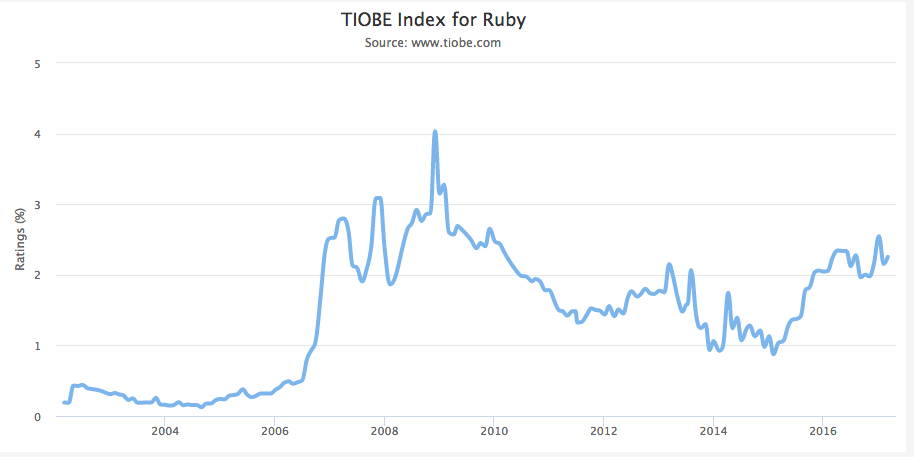
\includegraphics[width=1\linewidth]{obrazki/ruby_tiobe}
  \caption{Histora popularności języka Ruby według rankingu Tiobe}
  \label{fig:ruby_tiobe}
\end{figure}

\section{Istniejące systemy GIS w~języku Ruby}

\subsection{OpenStreetMap}

  OpenStreetMap jest internetowym systemem informacji geograficznej z~otwartym kodem źródłowym. System zbudowany z~wykorzystaniem bazy danych PostgreSQL, frameworku Ruby on Rails oraz biblioteki javascriptowej Leaflet służącej do tworzenia interaktywnych widoków z~mapami. Dostęp do danych jest otwarty, dane mogą być edytowane przez dowolnego użytkownika, dlatego mogą być niezgodne z~rzeczywistością. OpenStreetMap definiuje 4 typy obiektów przestrzennych\cite{doc_osm}:
  \begin{itemize}
    \item Węzeł (ang. node) - pojedynczy punkt geoprzestrzenny reprezentowany przez długość i~szerokość geograficzną.
    \item Linia (ang. way) - jest to uporządkowany zbiór punktów, które mogą reprezentować funkcje liniowe(wektory) lub obszary.
    \item Relacja (ang. relation) - składa się z~uporządkowanej listy węzłów, linii i~innych relacji.
    \item Tag (ang. tag) - to jednostka informacji dołączona do obiektu jednego z~powyżej opisanych typów. Tag składa się z~klucza oraz wartości. 
  \end{itemize}

  OpenStreetMap można wykorzystać przez utworzenie komponentu HTML z~wybraną mapą, gotowego do zamieszczenia na dowolnej stronie internetowej lub przez pobranie danych z~wybranej mapy. Skompresowane aktualne dane dla całej planety z~pojedynczego dnia zajmują prawie 40GB. Można pobierać również dane historyczne.

\subsection{MangoMap}

  MangoMap jest komercyjnym narzędziem do tworzenia map dostępnych przez internet z~własnych danych geoprzestrzennych. Ceny za korzystanie z~serwisu wynoszą 49-399\$ miesięcznie w~zależności od ilości map i~udostępnianego miejsca na serwerze do przechowywania danych. System zbudowany jest w~oparciu o~framework Ruby on Rails. Mapy tworzy się przy użyciu interfejsu graficznego. Stworzone mapy mogą być udostępnione na serwerze MangoMap przez unikalny link lub zamieszczone na zewnętrznej stronie WWW przez komponent HTML\cite{doc_mango}.

\chapter{Frameworki internetowe w~języku Ruby}

"Framework" można zdefiniować jako szkielet służący do budowania aplikacji, czyli zbiór gotowych rozwiązań powtarzających się problemów i~wzór do budowania nowych funkcjonalności.\cite{framework}

W języku Ruby istnieje kilkanaście wspieranych frameworków internetowych. Wybór wykorzystanych frameworków w~niniejszej pracy dokonano w~następujący sposób:
  \begin{enumerate}
    \item Podzielono frameworki według daty opublikowania pierwszej wersji na 3 grupy:
    \begin{enumerate}
      \item opublikowane w~latach 2004 - 2010 - frameworki o~ugruntowanej pozycji
      \item opublikowane w~latach 2011 - 2015 - stosunkowo nowe frameworki
      \item opublikowane w~latach 2016 - 2017 - najnowsze frameworki
    \end{enumerate}
    \item z~każdej grupy wybrano framework z~największą ilością pobrań.
  \end{enumerate}
Ta metoda ma na celu wyłonienie najpopularniejszych frameworków, które powstały w~różnych etapach języka Ruby, jednocześnie każdy z~nich współpracuje z~najnowszą wersją języka. w~ten sposób wybrano \emph{Ruby on Rails, Trailblazer i~Hanami.}


\begin{table}[H]
  \caption{ Frameworki internetowe w~języku Ruby \protect\footnotemark}
  \centering
  \begin{tabularx}{1\linewidth}{|X|X|X|X|} \hline
    Nazwa & Data opublikowania \newline pierwszej wersji & Data opublikowania \newline  najnowszej wersji & Ilość pobrań \\ \hline
    \rowcolor{lightgray}
    Ruby on Rails & 25.10.2004 r. & 20.03.2017 r. & 91 898 706 \\ \hline
    Hobo & 29.04.2007 r. & 07.05.2016 r. & 211 042 \\ \hline
    Sinatra & 04.10.2007 r. & 19.03.2017 r. & 45 207 501 \\ \hline
    Padrino & 16.11.2009 r. & 23.03.2017 r. & 556 481 \\ \hline
    Cuba & 25.04.2010 r. & 01.07.2016 r. & 124 371 \\ \Xhline{4\arrayrulewidth}
    Strelka & 24.08.2011 r. & 19.01.2017 r. & 57 007 \\ \hline
    Pakyow & 20.09.2011 r. & 15.07.2016 r. & 18 222 \\ \hline
    Scorched & 03.03.2013 r. & 12.10.2016 r. & 26 929 \\ \hline
    \rowcolor{lightgray}
    Trailblazer & 26.07.2013 r. & 23.01.2017 r. & 96 217 \\ \hline
    Vanilla & 09.05.2015 r. & 05.07.2016 r. & 80 125 \\ \Xhline{4\arrayrulewidth}
    \rowcolor{lightgray}
    Hanami & 20.01.2016 r. & 06.04.2017 r. & 28 885 \\ \hline
    Dry-web & 21.04.2016 r. & 02.02.2017 r. & 7 190 \\ \hline
  \end{tabularx}
\end{table}
\footnotetext{Zestawienia przygotowano na podstawie danych z~https://rubygems.org/ oraz https://www.ruby-toolbox.com. Pominięto frameworki, których ostatnia wersja ukazała się ponad rok temu. Aktualne na dzień 08.04.2017 r.}

\section{Ruby on Rails}

Pierwsza stabilna wersja (1.0.0) frameworku Ruby on Rails ukazała się pod koniec 2005 roku, aktualna wersja (5.0.2) została opublikowana 02.03.2017 r. Aplikacja zbudowana z~wykorzystanie RoR jest oparta o~wzorzec projektowy Model-Widok-Kontroler\cite{rails_agile} (ang. Model-View-Controller). Aplikacja oparta na tym wzorcu jest podzielona na 3 części:
\begin{itemize}
  \item Modele (ang. model) - reprezentują logikę biznesową. w~tej warstwie znajdują się wszelkie obiekty, które służą do wykonywania operacji związanych z~implementacją funkcjonalności aplikacji.
  \item Widoki (ang. view) - służą do prezentowania danych. 
  \item Kontrolery (ang. controller) - obsługują zapytania użytkownika. Nie zawierają w~sobie żadnej logiki biznesowej.
\end{itemize}

\begin{figure}[H]
  \centering
  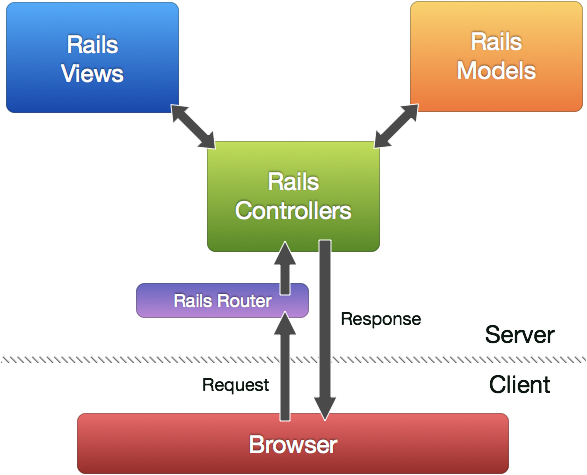
\includegraphics[width=1\linewidth]{obrazki/rails_mvc}
  \caption{Architektura aplikacji w~Ruby on Rails, źródło: http://blog.ifuturz.com/ruby-on-rails/ruby-on-rails-mvc-learn-with-fun.html}
  \label{fig:rails_mvc}
\end{figure}
\newpage
Dwie główne zasady frameworku\cite{doc_rails}:

\begin{itemize}
  \item Nie powtarzaj się (ang. Don't Repeat Yourself) - każda informacja powinna mieć pojedynczą, jednoznaczną i~autorytatywną reprezentacje w~kodzie źródłowym systemu. Ułatwia to utrzymywanie kodu.
  \item Konwencja ponad konfiguracje (ang. Convention Over Configuration) - RoR posiada ustalone zasady postępowania w~różnych przypadkach. Aplikacja domyślnie zachowuje się według tych zasad, nie wymagając dodatkowej konfiguracji. Pozwala to zredukować ilość kodu źródłowego.
\end{itemize}


\begin{figure}[H]
  \centering
  \begin{forest}
    for tree={
      font=\ttfamily,
      grow'=0,
      child anchor=west,
      parent anchor=south,
      anchor=west,
      calign=first,
      edge path={
        \noexpand\path [draw, \forestoption{edge}]
        (!u.south west) +(7.5pt,0) |- node[fill,inner sep=1.25pt] {} (.child anchor)\forestoption{edge label};
      },
      before typesetting nodes={
        if n=1
          {insert before={[,phantom]}}
          {}
      },
      fit=band,
      before computing xy={l=15pt},
    }
    [project\_root
      [app
        [controllers]
        [models]
        [views]
      ]
    ]
  \end{forest}
  \caption{Podstawowa struktura projektu Ruby on Rails}
  \label{fig:rails_structure}
\end{figure}


\section{Trailblazer}

Trailblazer w~dużej części bazuje na Ruby on Rails, posiada wiele wspólnych bibliotek. Framework w~stabilnej wersji(1.0.0) został opublikowany 25.08.15 r., aktualna wersja(2.0.3) ukazała się 23.01.2017 r. Trailblazer wykorzystuje architekturę MVC z~dodatkowymi warstwami abstrakcji\cite{nick_trailblazer}:

\begin{itemize}
  \item Kontroler (ang. controller) - służy tylko do obsługi zapytań HTTP, nie posiada w~sobie żadnej logiki przetwarzania danych.
  \item Operacja (ang. operation) - skupia w~sobie całą logikę biznesową i~jest podzielona na:
  \begin{itemize}
    \item Formularz (ang. form) - odpowiada za walidacje danych wejściowych operacji.
    \item Reprezentant (ang. representer) - służy do rzutownia otrzymanych danych z~kontrolera do postaci modelu oraz w~drugą stronę do zmiany modelu na postać akceptowana przez kontroler.
    \item Model (ang. model) - reprezentuje obiekt zapisywany w~bazie danych, nie zawiera w~sobie żadnej logiki, jedynie konfiguracje.
  \end{itemize}
  \item Komórki (ang. cells) - przygotowują dane do prezentacji.
  \item Widok (ang. view) - prezentuje dane.
\end{itemize}

\begin{figure}[H]
  \centering
  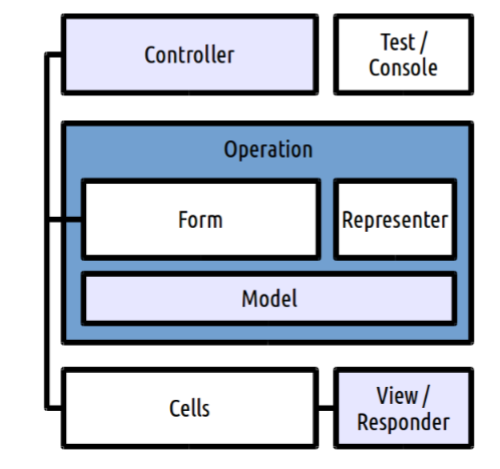
\includegraphics[width=1\linewidth]{obrazki/trailblazer_architecture}
  \caption{Architektura aplikacji w~Trailblazer}
  \label{fig:trailblazer_architecture}
\end{figure}

Framework Trailblazer jako główne zadanie obrał utrzymywanie rozbudowanych aplikacji, dzięki dobrze skalującej się architekturze. Dobrze integruje się z~innymi frameworkami Rubiego takimi jak Ruby on Rails, Hanami, Sinatra pozwalając na refaktoryzacje używanych produkcyjne aplikacji małymi krokami.

\begin{figure}[H]
  \centering
  \begin{forest}
    for tree={
      font=\ttfamily,
      grow'=0,
      child anchor=west,
      parent anchor=south,
      anchor=west,
      calign=first,
      edge path={
        \noexpand\path [draw, \forestoption{edge}]
        (!u.south west) +(7.5pt,0) |- node[fill,inner sep=1.25pt] {} (.child anchor)\forestoption{edge label};
      },
      before typesetting nodes={
        if n=1
          {insert before={[,phantom]}}
          {}
      },
      fit=band,
      before computing xy={l=15pt},
    }
    [project\_root
      [app
        [concepts
          [item
            [cell]
            [contract]
            [lib]
            [operation]
            [views]
          ]
          [item2
            [cell]
            [contract]
            [lib]
            [operation]
            [views]
          ]
        ]
      ]
    ]
  \end{forest}
  \caption{Podstawowa struktura projektu Trailblazer}
  \label{fig:trailblazer_structure}
\end{figure}

\section{Hanami}

Hanami jest lekkim frameworkiem internetowym opartym o~architekturę MVC, zbudowanym z~wielu mikro-bibliotek. w~przeciwieństwie do Ruby on Rails, Hanami nie stawia konwencji ponad konfiguracje, wszystkie informacje powinny być zawarte w~napisanym przez programistę kodzie, którego zrozumienie nie wymaga znajomości konwencji frameworka. Architekura projektu jest głównie inspirowana przez te dwa podejścia:

\begin{itemize}
  \item Czysta architektura (ang. clean architecture) - schemat tej architektury składa się z~kolejnych zawierających się w~sobie kół. Każde wewnętrzne koło nie ma żadnych zależności w~zewnętrznym kole, czyli w~obiektach należących do wewnętrznego koła, nie ma odwołań do obiektów z~zewnętrznych kół\cite{clean_architecture}. To podstawowa zasada tego podejścia. 

  \begin{figure}[H]
    \centering
    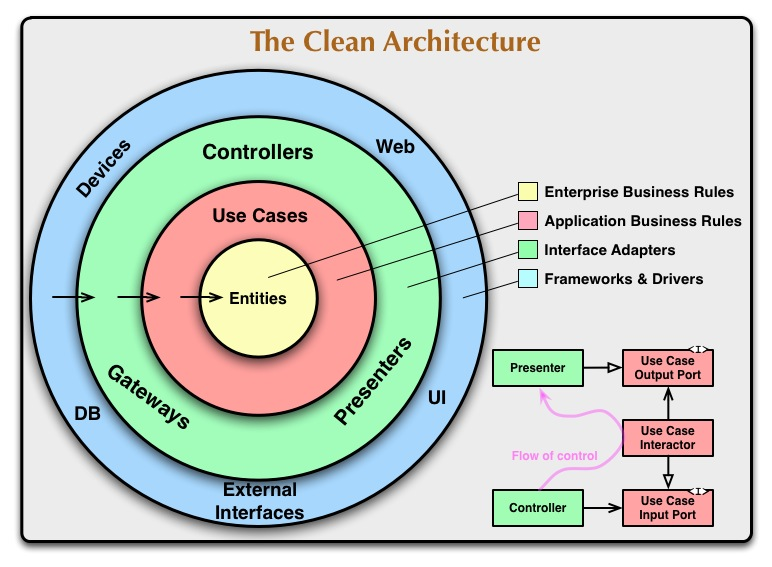
\includegraphics[width=1\linewidth]{obrazki/clean_architecture}
    \caption{Schemat czystej architektury}
    \label{fig:clean_architecture}
  \end{figure}

  Na schemacie \ref{fig:clean_architecture} można wyróżnić 4 byty:

  \begin{itemize}
    \item Encje (ang. entities) - zawierają ogólne reguły biznesowe systemu. Mogą być reprezentowane przez obiekty z~metodami, struktury danych lub pojedyncze funkcje.
    \item Przypadki użycia (ang. use cases) - ta warstwa skupia w~sobie wszystkie możliwe przypadki użycia systemu przez użytkownika. Znajduje się tu cała logika biznesowa zarządzania encjami. Zmiana w~tej warstwie nie powinna wpływać na encje, interfejs użytkownika lub bazę danych.
    \item Adaptery interfejsów (ang. interface adapters) - na tym poziomie dane są konwertowane z~formatu najbardziej dogodnego dla przypadków użycia i~encji do formatu przyjmowanego przez zewnętrzne narzędzia takie jak baza danych lub przeglądarka internetowa. 
    \item Frameworki oraz narzędzia (ang. frameworks and drivers) - w~tej warstwie znajdują się zewnętrzne narzędzia takie jak inne frameworki, baza danych lub przeglądarka internetowa.
  \end{itemize}

  \item Najpierw monolit (ang. monolith first) - według tej zasady budowę systemu zaczyna się od monolitycznej aplikacji. Jednak budowa aplikacji od samego początku powinna być jak najbardziej modularna aby można było ją później rozbić na wiele mniejszych aplikacji.

  Zgodnie z~zasadą \emph{czystej architektury} w~utworzonym projekcie systemu z~użyciem Hanami oddzielona jest warstwa logiki biznesowej znajdująca się w~folderze \emph{lib\\} projektu od mechanizmu komunikacji z~innymi serwisami zawartego w~folderze \emph{apps\\}.

  Hanami posiada kontener aplikacji, który pozwala nam utworzyć wiele aplikacji w~ramach jednego projektu, które korzystają z~tego samego zbioru encji i~przypadków użycia, a~następnie uruchomić je w~jednym procesie Rubiego.
\end{itemize}

\begin{figure}[H]
  \centering
  \begin{forest}
    for tree={
      font=\ttfamily,
      grow'=0,
      child anchor=west,
      parent anchor=south,
      anchor=west,
      calign=first,
      edge path={
        \noexpand\path [draw, \forestoption{edge}]
        (!u.south west) +(7.5pt,0) |- node[fill,inner sep=1.25pt] {} (.child anchor)\forestoption{edge label};
      },
      before typesetting nodes={
        if n=1
          {insert before={[,phantom]}}
          {}
      },
      fit=band,
      before computing xy={l=15pt},
    }
    [project\_root
      [apps
        [web
          [controllers]
          [templates]
          [views]
        ]
      ]
      [lib
        [main
          [entities]
          [repositories]
        ]
      ]
    ]
  \end{forest}
  \caption{Podstawowa struktura projektu Hanami}
  \label{fig:hanami_structure}
\end{figure}

\chapter{Narzędzia dostępne do przetwarzania danych geograficznych w~języku Ruby}
\section{Przechowywanie danych}
\subsection{PostGIS}
\subsection{MySQL Spatial}
\subsection{SpatiaLite}
\subsection{MongoDB}

\section{Przetwarzanie danych}
\subsection{Rgeo}
\subsection{GeoRuby}

\section{Prezentowanie danych}
\subsection{Leaflet}
\subsection{GoogleMaps}



\chapter{Badanie wydajności przetwarzania danych geograficznych}
\section{Plan eksperymentów}
\emph{użyte narzędzia, metody mierzenia, przebieg badań}

\section{Wyniki badań}
\emph{zapis, odczyt, wyszukiwanie, aktualizacja}

\chapter{Porównianie funkcjonalności wybranych frameworków}

\chapter{Porównianie struktur wykonanych projektów}

\chapter{Podsumowanie}
\section{Analiza wyników badań}
\emph{który framework jest najbardziej wydajny w~rozpatrywanych przypadkach}

\section{Realizacja celu projektu}
\emph{czy cel projektu został zrealizowany, napotkane trudności/przeszkody}

\begin{thebibliography}{inz}
  \addcontentsline{toc}{chapter}{Literatura}

  \bibitem{doc_rgeo}
  \emph{Dokumentacja biblioteki Rgeo}, dostępna pod adresem:\\ \url{http://www.rubydoc.info/gems/rgeo/}, aktualne na dzień 08.03.2017r.

  \bibitem{doc_hanami}
  \emph{Dokumentacja Hanami}, dostępna pod adresem:\\ \url{http://hanamirb.org/guides/}, aktualne na dzień 08.03.2017r.

  \bibitem{doc_ruby}
  \emph{Dokumentacja języka Ruby}, dostępna pod adresem:\\ \url{https://www.ruby-lang.org/pl/documentation/}, aktualne na dzień 08.03.2017r.

  \bibitem{doc_mango}
  \emph{Dokumentacja MangoMap}, dostępna pod adresem:\\ \url{http://help.mangomap.com/}, aktualne na dzień 22.04.2017r.

  \bibitem{doc_osm}
  \emph{Dokumentacja OpenStreetMap}, dostępna pod adresem:\\ \url{http://wiki.openstreetmap.org/}, aktualne na dzień 08.03.2017r.

  \bibitem{doc_postgis}
  \emph{Dokumentacja PostGIS}, dostępna pod adresem:\\ \url{http://postgis.net/documentation/}, aktualne na dzień 08.03.2017r.

  \bibitem{doc_rails}
  \emph{Dokumentacja Ruby on Rails}, dostępna pod adresem:\\ \url{http://guides.rubyonrails.org/}, aktualne na dzień 08.03.2017r.

  \bibitem{doc_trailblazer}
  \emph{Dokumentacja Trailblazer} https://8thlight.com/blog/uncle-bob/2012/08/13/the-clean-architecture.html

  \bibitem{principles_gis}
  Huisman Otto, By (de) Rolf A., \emph{Principles of Geographic Information Systems}, ITC, 2009

  \bibitem{clean_architecture}
  Martin Robert, \emph{The Clean Architecture}, dostępna pod adresem:\\ \url{https://8thlight.com/blog/uncle-bob/2012/08/13/the-clean-architecture.html}, aktualne na dzień 20.04.2017r.

  \bibitem{rails_agile}
  Ruby Sam, Thomas Dave, Hansson Heinemeier David, \emph{Agile Web Development with Rails 5}, Pragmatic Programmers, 2016

  \bibitem{gis_introduction}
  Schmandt Michael, \emph{GIS Commons: An Introductory Textbook on Geographic Information Systems}, dostępne pod adresem:\\
  \url{http://giscommons.org/}, aktualne na dzień 07.04.2017r.

  \bibitem{framework}
  Smyrdek Przemysław, \emph{Czym jest framework i~po co go używać}, dostępne pod adresem:\\
  \url{http://poznajprogramowanie.pl/czym-jest-framework-i-po-co-go-uzywac/}, aktualne na dzień 20.04.2017r.
  
  \bibitem{nick_trailblazer}
  Sutterer Nick, \emph{Trailblazer. a~New Architecture For Rails}, Leanpub, 2016
  
 
\end{thebibliography}

\end{document}